\documentclass{beamer}
\usepackage[french]{babel}
\mode<presentation>
\usepackage[utf8]{inputenc}

\usepackage{listings}
\definecolor{colKeys}{rgb}{0,0,1}
\definecolor{colIdentifier}{rgb}{0,0,0}
\definecolor{colComments}{rgb}{0,0.5,1}
\definecolor{colString}{rgb}{0.6,0.1,0.1}

\lstset{language=[x86masm]Assembler}
\lstset{%configuration de listings
float=hbp,%
basicstyle=\ttfamily\small, %
identifierstyle=\color{colIdentifier}, %
keywordstyle=\color{colKeys}, %
stringstyle=\color{colString}, %
commentstyle=\color{colComments}, %
columns=flexible, %
tabsize=2, %
extendedchars=true, %
showspaces=false, %
showtabs=false, %
showstringspaces=false, %
%numbers=left, % Numerotation des lignes
%numberstyle=\tiny, %
breaklines=true, %
breakautoindent=true, %
captionpos=b,%
%xrightmargin=-2cm, %
%xleftmargin=-2cm
}
%%%%%%%%%%%%%%%%%%%%%%% 	  	

\usetheme{Luebeck}
%\usecolortheme{seahorse}
\setbeamertemplate{bibliography item}[text]
\setbeamertemplate{blocks}[rounded][shadow=true]


%%%%%%%%%%%%LISTING


%%%%%%%%%%%%%%%%%


\title[Introduction  la sécurité informatique]{Introduction à la virologie informatique: principes, attaques et défenses}
\institute{\textbf{Pierre Ramet:} \texttt{ramet@labri.fr}}


\author{DUT S4}
\date{2013-2014}

%\setcounter{tocdepth}{1}
\begin{document}

\begin{frame}

  \titlepage

\end{frame}

\AtBeginSubsection[]
                  {
                    \begin{frame}<beamer>
                      \frametitle{Plan}
                      \tableofcontents[currentsection,currentsubsection,sectionstyle=show/shaded,subsectionstyle=show/shaded/hide]
                    \end{frame}
                  }

\section{Introduction}
\subsection{Introduction}

\begin{frame}{Introduction}

\begin{definition}
"A virus is a program that is able to infect other programs by modifying them to include a possibly evolved copy of itself." \\
\hfill \textit{F.Cohen}
\end{definition}
\begin{itemize}
\item Virus !=malware
\item Nous ne \textbf{parlerons pas} des vers (trivial)
\item Programmes souvent écrits en assembleur (entre 10 lignes et 20000 lignes de code)
\item Grande variété de virus:
\begin{itemize}
\item Différentes cibles
\item Différentes charges malicieuses
\item Différents vecteurs de propagations
\end{itemize}
\end{itemize}
\end{frame}

\begin{frame}{Corewar}
\begin{itemize}
\item Un exemple simple
\begin{itemize}
\item Machine virtuelle minimaliste
\item Deux programmes s'affrontent pour \textit{coloniser} la mémoire
\item Le code vit dans la mémoire
\end{itemize}
\item Exemple: corewar
\end{itemize}
\begin{figure}[!ht]
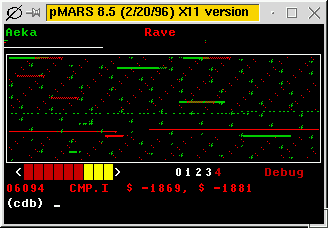
\includegraphics[scale=0.5]{corewar.png}
\center
\caption{Le jeu de la vie}
\end{figure}

\end{frame}


\subsection{Objectif du cours}
\begin{frame}{Pourquoi les étudier ?}
\begin{itemize}
\item C'est la plus ancienne nuisance informatique
\item La \textbf{quasi totalité des techniques} des rootkits, vers, trojan et shellcodes \textbf{sont issues des virus}
\item Un peu plus que de simples \texttt{format c:}
\begin{itemize}
\item Théorie des langages
\item Programmation système
\item Reverse engineering et obfuscation
\item et bien d'autres ...
\end{itemize}
\item Le problème de détection d'un virus est \textbf{indécidable}
\begin{itemize}
\item Preuve de F.Cohen basée sur l'arrêt d'une machine de Turing
\end{itemize}
\end{itemize}
\end{frame}

\begin{frame}{Pourquoi les étudier ? (2)}
Parce qu'ils sont dangereux !
\begin{itemize}
\item Remet en jeu l'\textbf{intégrité} et la {disponibilité} du Système Informatique:
\begin{itemize}
\item Suppression de fichiers
\item Backdoors
\item Charge réseau (Netsky)
\item Ransomwares (Gpcode)
\end{itemize}
\item Parfois la \textbf{confidentialité}:
\begin{itemize}
\item Vols de mots de passe (jeux en ligne, banque en ligne, etc.)
\end{itemize}
\item Augmentation du nombre de postes connectés et de médias amovibles
\end{itemize}
\end{frame}

\begin{frame}{Pourquoi les étudier ? (3)}
Situation actuelle:
\begin{itemize}
\item Marché éclaté entre plus de 20 marques ( 3 leaders : McCafee, Symantec et Trend Micro)
\item Marché en progression (+12,5\% en 2008)
\item Collaboration entre les différents éditeurs
\item Plus de 100 nouvelles détections par jour
\item ... et toujours \textbf{pas d'antivirus parfait} (\textit{cf. Vigard})
\end{itemize}
\end{frame}



\begin{frame}{Objectifs de ce cours}
\begin{itemize}
\item Culture générale du spécialiste en sécurité
\item Effacer les idées préconcues
\item Tracer un historique rapide de l'évolution de la virologie informatique
\begin{itemize}
\item Un bon aperçu du monde de la sécurité informatique
\end{itemize}
\item Introduction aux technique d'infection et de mutation de code
\begin{itemize}
\item Polymorphisme, métamorphisme, chiffrement de code, anti-émulation
\item Se retrouvent dans tous les malwares actuels
\end{itemize}
\item Appréhender les techniques de détection de virus
\begin{itemize}
\item Signature, émulation, heuristique, code normalization, détection comportementale
\end{itemize}
\end{itemize}
\end{frame}


\begin{frame}{Contenu du cours}
\begin{itemize}
\item Historique de la virologie informatique
\begin{itemize}
\item du point de vue de l'attaquant
\item du point de vue du défenseur
\end{itemize}
\item Quelques notions théoriques
\begin{itemize}
\item Théorie des langages, Chomsky hierarchy
\item Il existe des approches très formelles de la virologie que nous n'aborderons pas (cf. Fillol)
\end{itemize}
\item Revue des principales techniques d'obfuscation
\begin{itemize}
\item chiffrement du code, polymorphisme, métamorphisme, anti-*
\end{itemize}
\item TP sur machine virtuelle Windows
\begin{itemize}
\item écriture d'une routine de chiffrement pour un virus existant
\item écriture de règles de polymorphisme
\item test de détection sur un AV récent
\end{itemize}
\end{itemize}
\end{frame}




\section{Première génération: les virus de boot}
\subsection{Méthode d'infection}

\begin{frame}{Le premier virus informatique}
\begin{itemize}
\item Les virus de boot sont les 1er virus informatique qui se sont propagés
\item En 1986: le virus Brain
\item Avantage: indépendant de l'O.S (surtout à l'époque !)
\item Démarrage du virus avant l'O.S
\end{itemize}
\end{frame}



\begin{frame}{Le virus Brain}
\begin{figure}[!ht]
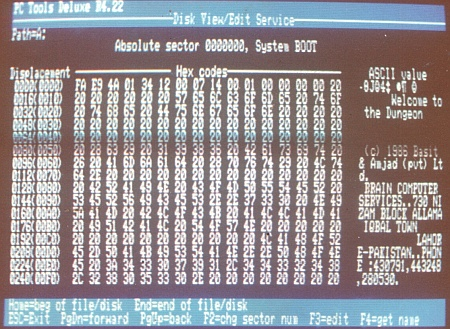
\includegraphics[scale=0.5]{brain.jpg}
\center
\caption{Le virus brain}
\end{figure}
\end{frame}

\begin{frame}{Fonctionnement}
\begin{itemize}
\item Il n'est pas possible de charger l'O.S depuis la ROM
\item Au démarrage du PC, le premier secteur du disque dur (le MBR) est chargé en mémoire 
\item Le MBR contient  un \textit{bootstrap loader} qui charge la partiton active depuis la table de partitions
\item La partition active contient le code de chargement de l'O.S
\end{itemize}
\end{frame}

\begin{frame}{Le MBR}
\begin{figure}[!ht]
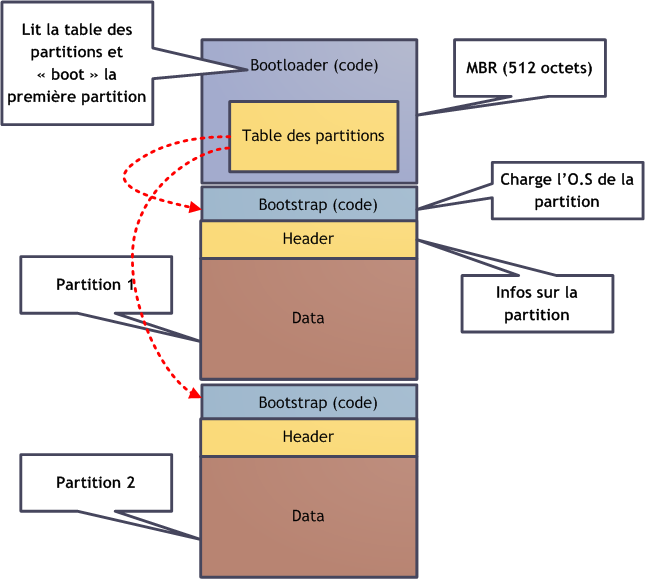
\includegraphics[scale=0.3]{boot.png}
\center
\caption{Démarrage d'un PC}
\end{figure}
\end{frame}


\begin{frame}{Les types d'infections du MBR}
\begin{itemize}
\item Remplacement du bootstrap (\textit{Stoned)}
\begin{itemize}
\item Déplacement de la table de partitions (fin du MBR ou espace libre du disque)
\item Insertion du code à la place du bootstrap
\end{itemize}
\item Remplacement du MBR (\textit{Azura 91)}
\begin{itemize}
\item Pas de sauvegarde de la table de partitions (plus d'espace)
\item Chargement de la partition active par le virus
\end{itemize}
\item Modification de la table de partition (\textit{Starship})
\begin{itemize}
\item La table de partitions est parsée et modifiée
\item Chargement d'un secteur différent, où est situé le virus
\end{itemize}
\end{itemize}
\end{frame}

\begin{frame}{Vecteur de propagation}
\begin{itemize}
\item A l'époque, les programmes étaient distribués sous forme de disquette bootable
\begin{itemize}
\item Pas vraiment d'OS
\end{itemize}
\item On s'échangeait des programmes en recopiant des disquettes
\item Les virus de boot:
\begin{itemize}
\item Se chargeaient en mémoire au démarrage de l'ordinateur
\item Repéraient la routine du BIOS chargée d'écrire sur une disquette (\texttt{int 13h)}
\item \textbf{Détournaient} cette routine vers du code viral
\item Lorsque cette routine était appelée:
\begin{itemize}
\item Écriture des données demandées
\item ... puis écriture du virus sur le MBR
\end{itemize}
\end{itemize}
\end{itemize}
\end{frame}



\begin{frame}{Propagation des virus MBR}
\begin{figure}[!ht]
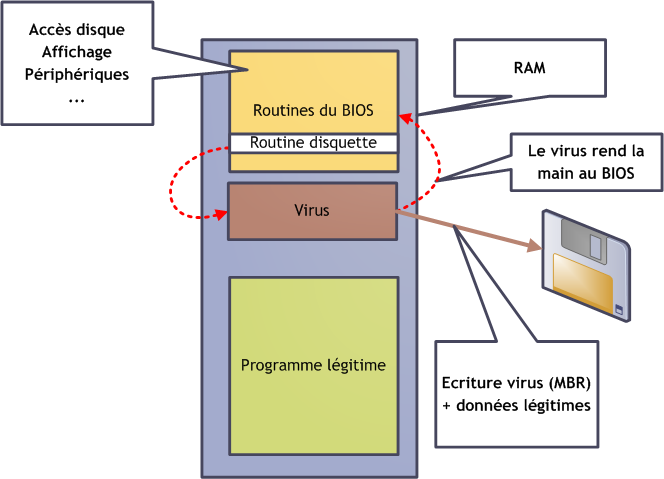
\includegraphics[scale=0.3]{mbr.png}
\center
\caption{Propagation d'un virus type MBR}
\end{figure}

\end{frame}

\subsection{Actualité}
\begin{frame}{Et maintenant ? }
Les virus Autorun sont les descendants actuels des virus de boot
\begin{itemize}
\item Sous Windows, lorsqu'un disque amovible est inséré, le fichier \texttt{autorun.inf} est examiné
\begin{block}{Autorun}
\texttt{
[autorun]\\
OPEN=virus.doc.exe\\
ICON=msword.ico\\
...
}
\end{block}
\item Une fois le virus lancé, il scannera en permanence la présence de disques amovibles
\begin{itemize}
\item Pour y ajouter virus.exe et autorun.inf
\item En fichier caché bien sur
\end{itemize}
\item Encore plus simple qu'avant !
\item Et toujours aussi efficace ! (cf. \textit{Seagate})
\end{itemize}
\end{frame}


\subsection{Détection}

\begin{frame}{Première génération: les scanners artisanaux}
\begin{itemize}
\item Pas encore de société d'antivirus
\item Souvent, un antivirus différent pour chaque virus
\item Apparition de la recherche par signature

\begin{figure}[!ht]
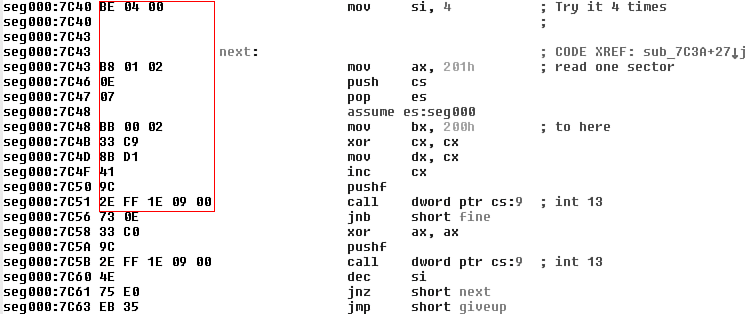
\includegraphics[scale=0.4]{stoned.png}
\center
\caption{Signature sur le virus Stoned}
\end{figure}

\end{itemize}
\end{frame}

\begin{frame}{La recherche par signature}
\begin{itemize}
\item Architecture de Von Neumann: code $\simeq$ données
\item Un programme binaire peut être vu comme un fichier quelconque
\item Les premiers antivirus:
\begin{itemize}
\item Lecture du MBR
\item Recherche d'une signature simple (on ne parle même pas de regexp)
\item Si signature trouvée $\rightarrow$ alerte ou réparation du MBR
\end{itemize}
\item Un antivirus ne ciblait qu'un ou deux virus
\item Acceptable, car moins d'une dizaine de nouveaux virus par an
\end{itemize}
\end{frame}

\section{Deuxième génération: les infecteurs de fichier}
\subsection{Fonctionnement}

\begin{frame}{Les infecteurs de fichiers}
Les infecteurs de fichiers exécutables
\begin{itemize}
\item Même fonctionnement que les virus biologiques
\item Virus informatiques les plus répandus
\item De nombreuses cibles:
\begin{itemize}
\item PE-exe, ELF, bat, sh, .py, .vbs
\end{itemize}
\item De nombreuses méthodes d'infection:
\begin{itemize}
\item appenders, prependers, cavity infectors, compagnons
\end{itemize}
\end{itemize}
\end{frame}

\begin{frame}{Principe général}
Les infecteurs de fichiers:
\begin{itemize}
\item Un exécutable est un fichier standard avec un format défini 
\begin{itemize}
\item Format PE: \url{http://www.microsoft.com/whdc/system/platform/firmware/PECOFF.mspx}
\item Format ELF: \url{http://www.asm-x86.fr/le-format-elf_a8}
\end{itemize}
\item Il est tout à fait légal de créer/modifier un fichier exécutable
\begin{itemize}
\item \texttt{gcc}, \texttt{patch}, \texttt{ld}
\end{itemize}
\item Il est ainsi possible d'\textbf{ajouter} et de \textbf{modifier} le code d'un programme
\end{itemize}
\end{frame}


\begin{frame}{Infection d'un exécutable}
\begin{itemize}
\item Comment infecter un fichier exécutable ?
\end{itemize}
\begin{figure}[!ht]
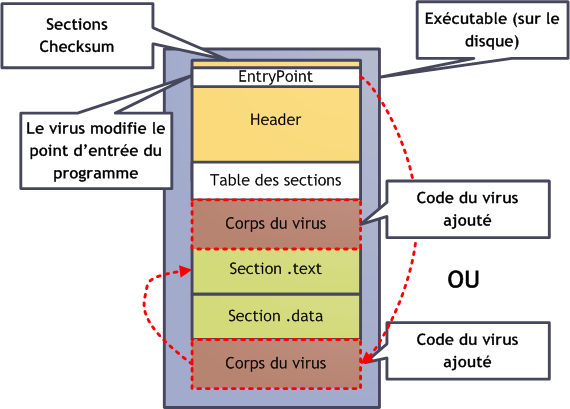
\includegraphics[scale=0.3]{infection.png}
\center
\caption{Infection d'un exécutable}
\end{figure}

\end{frame}





\begin{frame}{Spécificités}

\begin{itemize}
\item Le code du virus doit être \textit{position independant}
\begin{itemize}
\item Difficile de savoir où l'exécutable sera chargé (ASLR ...)
\end{itemize}
\item Il faut modifier l'exécutable hôte pour y insérer le virus
\begin{itemize}
\item Conserver la cohérence de la structure du fichier (checksum, en-têtes, ...)
\end{itemize}
\item \textit{Détournement} du flot de contrôle au sein de l'exécutable
\begin{itemize}
\item Modification de l'EP, per process residency, etc.
\end{itemize}
\item Plusieurs générations sur un même système hôte (proche du virus biologique)
\begin{itemize}
\item Possibilité de \textit{mutation} (polymorphisme, métamorphisme, ...)
\end{itemize}
\end{itemize}
\end{frame}

\subsection{Les différents types d'infection}

\begin{frame}{Les virus parasites}
\begin{columns}[t]
\begin{column}{4cm}
\begin{exampleblock}{Overwriting infectors}
\begin{itemize}
\item Virus déstructif
\item Le corps du virus est écrit \textbf{sur} le fichier hôte
\item Le virus, une fois exécuté, ne rendra pas la main 
\item Premiers infecteurs d'exes
\end{itemize}
\end{exampleblock}
\end{column}
\begin{column}{6cm}
\begin{figure}[!ht]
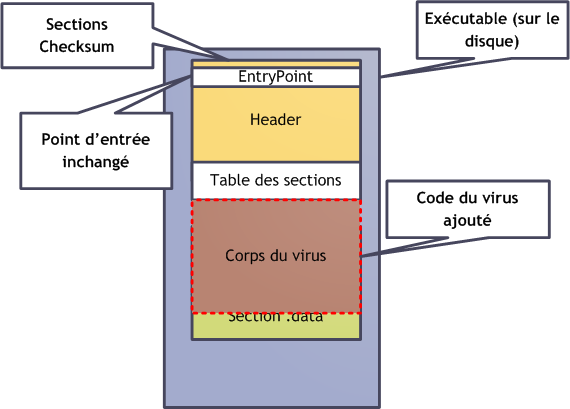
\includegraphics[scale=0.3]{overwriting.png}
\center
\end{figure}
\end{column}
\end{columns}

\end{frame}

\begin{frame}{Les virus parasites (2)}
\begin{columns}[t]
\begin{column}{4cm}
Avantages
\begin{itemize}
\item Extrêmement simples
\begin{itemize}
\item Infecte tous types de fichiers
\end{itemize}
\item Pas besoin de PIC
\begin{itemize}
\item C'est une copie d'exécutable
\end{itemize}
\end{itemize}
\end{column}
\begin{column}{5cm}
\item Inconvénients
\begin{itemize}
\item Détectable par l'utilisateur
\item Besoin de plus ?
\end{itemize}
\end{column}
\end{columns}
\begin{alertblock}{Exemple}
Les premiers virus DOS
\end{alertblock}
\end{frame}



\begin{frame}{Les infecteurs de header}
\begin{columns}[t]
\begin{column}{4cm}
\begin{exampleblock}{Header infectors}
\begin{itemize}
\item Code du virus très court
\item Inséré après les header de l'exécutable (padding)
\item Modification du point d'entrée
\end{itemize}
\end{exampleblock}
\end{column}
\begin{column}{6cm}
\begin{figure}[!ht]
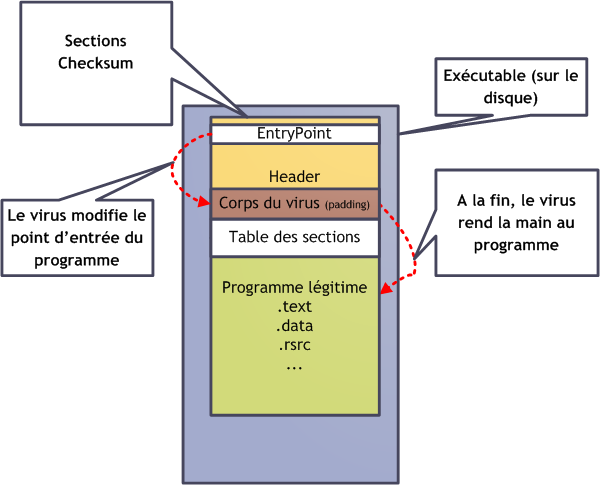
\includegraphics[scale=0.3]{header.png}
\center
\end{figure}
\end{column}
\end{columns}

\end{frame}

\begin{frame}{Les infecteurs de header (2)}
\begin{columns}[t]
\begin{column}{4cm}
Avantages
\begin{itemize}
\item Pas de modification de la taille du fichier
\begin{itemize}
\item Contre les whitelists
\end{itemize}
\item Pas de création/modification des sections
\begin{itemize}
\item Contre les heuristiques les plus grossières
\end{itemize}
\end{itemize}
\end{column}
\begin{column}{5cm}
\item Inconvénients
\begin{itemize}
\item Corps du virus nécessairement très court
\item Pas toujours de padding (XP, Vista)
\end{itemize}
\end{column}
\end{columns}
\begin{alertblock}{Exemple}
Murky
\end{alertblock}
\end{frame}

\begin{frame}{Les infecteurs de cavité}
\begin{columns}[t]
\begin{column}{4cm}
\begin{exampleblock}{Cavity infectors}
\begin{itemize}
\item Code du virus assez court
\item Fragmenté en $N$ parties, liées entre elles par des \texttt{jmp}
\item Inséré dans les sections \textit{inutiles} (\texttt{.reloc}), dans le \textit{padding}
\item Modification du point d'entrée
\end{itemize}
\end{exampleblock}
\end{column}
\begin{column}{6cm}
\begin{figure}[!ht]
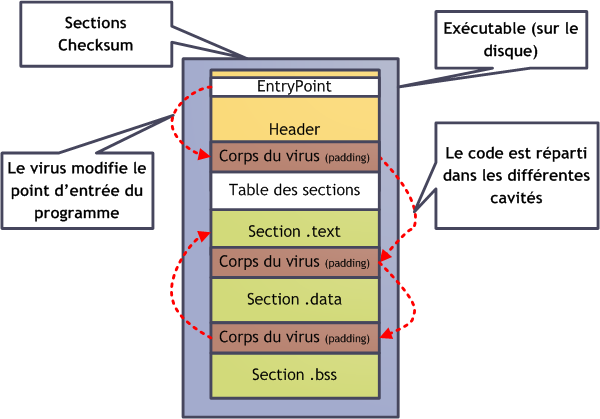
\includegraphics[scale=0.32]{cavite.png}
\center
\end{figure}
\end{column}
\end{columns}
\end{frame}


\begin{frame}{Les infecteurs de cavité (2)}
\begin{columns}[t]
\begin{column}{5cm}
Avantages
\begin{itemize}
\item Pas de modification de la taille du fichier
\begin{itemize}
\item Contre les whitelists
\end{itemize}
\item Pas de création/modification des sections
\begin{itemize}
\item Contre les heuristiques les plus grossières
\end{itemize}
\end{itemize}
\end{column}
\begin{column}{5cm}
Inconvénients
\begin{itemize}
\item Plus complexe (nécessite de reloger chaque partie)
\item Plus de place que pour l'infection de header, mais reste court (- de 4k)
\end{itemize}
\end{column}
\end{columns}
\begin{alertblock}{Exemple}
CIH, W2K/Installer 
\end{alertblock}
\end{frame}

\begin{frame}{Les infecteurs de fin/début de fichier}
\begin{columns}[t]
\begin{column}{4cm}
\begin{exampleblock}{File infectors}
\begin{itemize}
\item Code du virus arbitrairement long
\item Inséré en début ou fin de fichier
\item Modification de la table des sections
\item Modification du point d'entrée
\end{itemize}
\end{exampleblock}
\end{column}
\begin{column}{6cm}
\begin{figure}[!ht]
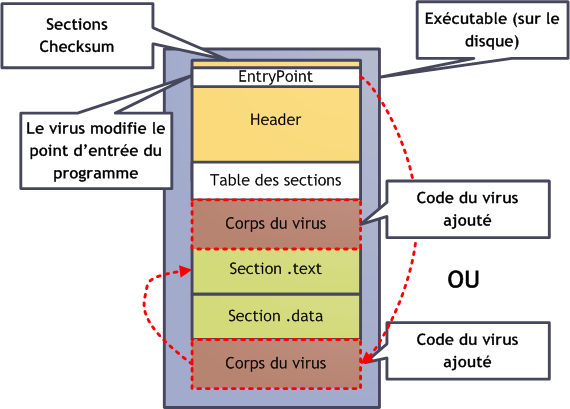
\includegraphics[scale=0.3]{appender.png}
\center
\end{figure}
\end{column}
\end{columns}
\end{frame}

\begin{frame}{Les infecteurs de début de fichier}
Infection en début de fichier
\begin{itemize}
\item Code du virus inséré \textbf{avant} la toute première section
\item Décalage de toutes les sections suivantes
\begin{itemize}
\item Nécessite les informations de relocation
\item Sauf si on utilise l'\textit{imagebase trick}
\end{itemize}
\item Plutôt discret (les heuristiques observent plus souvent la fin du fichier)
\end{itemize}
\end{frame}

\begin{frame}{Les infecteurs de fin de fichier}
Infection en fin de fichier
\begin{itemize}
\item Type d'infection le plus répandu
\item Code du virus inséré \textbf{après} la dernière section
\item Éventuellement, ajout d'une section supplémentaire
\item Moins discret que l'insertion à la fin du fichier
\begin{itemize}
 \item ... mais plus simple
\end{itemize}
\end{itemize}
\end{frame}


\begin{frame}{Les infecteurs de fin/début de fichier (2)}
\begin{columns}[t]
\begin{column}{5cm}
Avantages
\begin{itemize}
\item Portable
\begin{itemize}
\item Quasiment tous les exécutables peuvent être infectés par cette méthode
\end{itemize}
\item Simple à mettre en oeuvre
\item Corps du virus arbitrairement long
\end{itemize}
\end{column}
\begin{column}{5cm}
Inconvénients
\begin{itemize}
\item Modification 
\begin{itemize}
\item de la taille du fichier
\item de la table des sections
\item de l'entrypoint
\end{itemize}
\item Les antivirus regardent principalement la fin et le début des exécutable
\item Virus en un seul bloc
\begin{itemize}
\item signature plus aisée
\end{itemize}
\end{itemize}
\end{column}
\end{columns}
\begin{alertblock}{Exemple}
Anxiety, 90\% des virus
\end{alertblock}
\end{frame}

\begin{frame}{Les virus \textit{compresseurs}}
\begin{columns}[t]
\begin{column}{4cm}
\begin{exampleblock}{Compressing infectors}
\begin{itemize}
\item Code du virus relativement court
\item Inséré à la place du code de l'hôte
\item L'hôte est compressé (ZIP,LFZ ...)
\item ... et déplacé à la fin du fichier 
\end{itemize}
\end{exampleblock}
\end{column}
\begin{column}{6cm}
\begin{figure}[!ht]
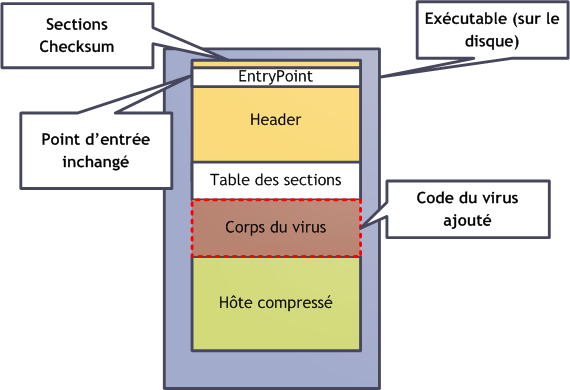
\includegraphics[scale=0.32]{zip.png}
\center
\end{figure}
\end{column}
\end{columns}
\end{frame}


\begin{frame}{Les virus \textit{compresseurs} (2)}
\begin{columns}[t]
\begin{column}{5cm}
Avantages
\begin{itemize}
\item Pas de modification de la taille du fichier
\begin{itemize}
\item Contre les whitelists
\end{itemize}
\item Virus non-PIC
\item Plus difficile à désinfecter
\end{itemize}
\end{column}
\begin{column}{5cm}
Inconvénients
\begin{itemize}
\item Plus complexe 
\item Code nécessairement plus petit 
\item Infection pas toujours possible
\end{itemize}
\end{column}
\end{columns}
\begin{alertblock}{Exemple}
W32/Redemption, W32/Aldebera
\end{alertblock}
\end{frame}


\begin{frame}{Démo}
\begin{alertblock}{Démonstration}
\begin{itemize}
\item Cible: Notepad
\item Différences avant/après infection
\end{itemize}
\end{alertblock}
\end{frame}

\subsection{Détection}

\subsubsection{Recherche par signature}
\begin{frame}{La recherche par signature}
\begin{itemize}
\item Scanner de première génération $\simeq$ FSA
\begin{itemize}
\item Code $\Leftrightarrow$ données
\item Signature $\Leftrightarrow$ expression régulière
\end{itemize}
\item Permet une détection exacte
\item Complexité ?
\item Un antivirus actuel contient plus de 100000 signatures
\end{itemize}
\end{frame}

\begin{frame}{La recherche par signature (2)}
\begin{figure}[!ht]
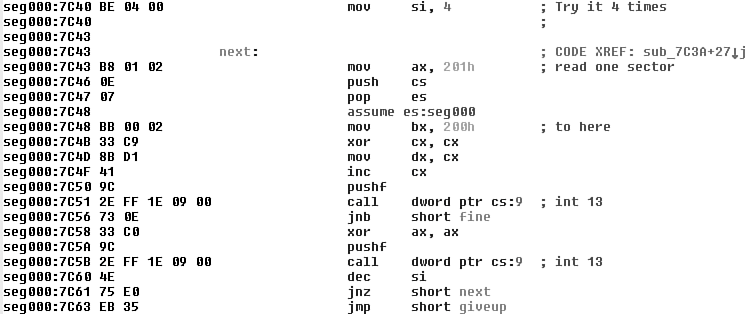
\includegraphics[scale=0.35]{stone.png}
\center
\caption{Stone: entrypoint}
\end{figure}
Signature: \texttt{0400 B801 020E 07BB 0002 33C9 8BD1 419C}
\end{frame}


\begin{frame}{La recherche par signature (3)}
Format des signatures
\begin{itemize}
\item Wildcards (joker) pour les virus \textbf{oligomorphiques}
\begin{exampleblock}{Exemple}
\texttt{0400 B801 020E 07BB ??02 \%3 33C9 8BD1 419C}
\end{exampleblock}
\item Mismatches
\begin{itemize}
\item mismatch de 2 $\Leftrightarrow$ autorise une distance <=2 entre chaque lexème du pattern
\end{itemize}
\item Bookmarks
\begin{itemize}
\item Zone de code stratégique du virus (OEP, clé de chiffrement)
\item Généralement utilisé pour la désinfection
\end{itemize}
\end{itemize}
\end{frame}


\begin{frame}{Optimisation de la recherche par signature}
\begin{itemize}
\item Filtrage de fichiers
\begin{itemize}
\item Ne considérer que les \texttt{*.exe}
\end{itemize}
\item Signature hashing
\begin{itemize}
\item Les X premiers octets de la signature sont hashés
\end{itemize}
\item Recherche localisée (smart scanning)
\begin{itemize}
\item En début, fin de fichier, à l'entrypoint
\end{itemize}
\item Smart scaning
\begin{itemize}
\item Ignorer les opcodes inutiles (nop, std ...)
\end{itemize}
\end{itemize}
\end{frame}

\subsubsection{Heuristique}
\begin{frame}{L'heuristique}
Vérification statique de la structure des exécutables :
\begin{itemize}
\item L'entrypoint est dans la dernière section ?
\item La dernière section est exécutable ?
\item Certains champs du header sont mal calculés ?
\item Une section .reloc ou .data reçoit le flot d'exécution ?
\item  Transfert du flot d'exécution d'une section à une autre ?
\item Apis suspectes importées (FindFistFile/FindNextFile/WriteFile ...) ?
\end{itemize}
\end{frame}

\begin{frame}[fragile]{Heuristique}
\begin{exampleblock}{Exemple de sortie d'un moteur heuristique}
\begin{lstlisting}[langage=java]
Analyzing SGWW2202.VXE
-Execution starts in last section
-Suspicious code section characteristics
-Virtual size is incorrect in header
-Suspicious relocation
-Suspicious code section 
-Using KERNEL32 address directly and looking for PE00
=> Possibly infected with an unknown Win32 virus (Level: 9)
\end{lstlisting}
\end{exampleblock}
\end{frame}

\section{Troisième génération: Chiffrement et polymorphisme}

\subsection{Le chiffrement de code}

\begin{frame}{Principe}
La mutation de code
\begin{itemize}
\item Technique de protection des virus
\item Objectif: éviter la détection par les \textbf{scanners}
\item Méthode: camoufler le code du virus
\item Moyens:
\begin{itemize}
\item Chiffrement
\item Oligomorphisme
\item Polymorphisme
\item Metamorphisme
\end{itemize}
\end{itemize}
\end{frame}


\begin{frame}{Le chiffrement}
\begin{columns}[t]
\begin{column}{5cm}
\begin{exampleblock}{}
\begin{itemize}
\item Technique simple: chiffrer le corps du virus
\item Le code du virus commence par un petit décodeur \textbf{en clair}
\begin{itemize}
\item Code constant
\item Clé embarquée, codée en dur
\item la clé \textbf{change à chaque génération}
\end{itemize}
\item Une fois déchiffré, saut vers le corps du virus
\end{itemize}
\end{exampleblock}
\end{column}
\begin{column}{5cm}
\begin{figure}[!ht]
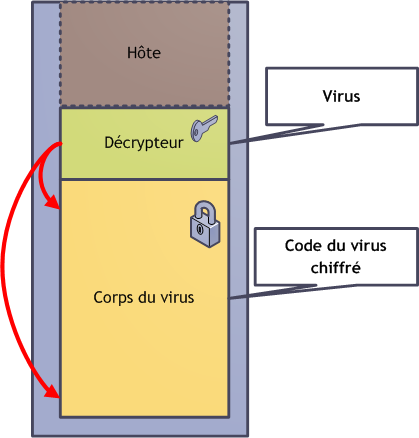
\includegraphics[scale=0.3]{chiffrement.png}
\center
\caption{Chiffrement de virus}
\end{figure}
\end{column}
\end{columns}
\end{frame}

\begin{frame}[fragile]{Le chiffrement (2)}
\begin{exampleblock}{Décrypteur du virus Mad}
\begin{lstlisting}
	mov edi, Start
	add edi, ebp
	mov ecx, 0A6Bh
	mov a1, [Key]
Decrypt :
	xor [edi], a1
	inc edi
	loop Decrypt
	jmp Start
Start :
; code du virus
\end{lstlisting}
\end{exampleblock}
\end{frame}

\begin{frame}{Le chiffrement (3)}
Technique plus avancées:
\begin{itemize}
\item Le décodeur peut changer de position 
\item Les décodeurs peuvent s'enchaîner (layers)
\item Utilisation d'API crypto
\item Le décodeur bruteforce la clé (\texttt{RDA fighter})
\end{itemize}
\end{frame}

\begin{frame}{A votre avis}
\begin{itemize}
\item \huge{Quelles contremesures possibles ?}
\end{itemize}
\end{frame}


\subsection{La mutation de code}
\begin{frame}{L'oligomorphisme}
\begin{columns}[t]
\begin{column}{5cm}
\begin{exampleblock}{Oligomorphisme}
\begin{itemize}
\item Le décodeur reste en clair
\item Utilisation de plusieurs décodeurs différents
\begin{itemize}
\item Whale 12, Memorial 96
\end{itemize}
\item Choix aléatoire d'un décodeur
\item Chaque décodeur est écrit par le vxer
\end{itemize}
\end{exampleblock}
\end{column}
\begin{column}{5cm}
\begin{figure}[!h]
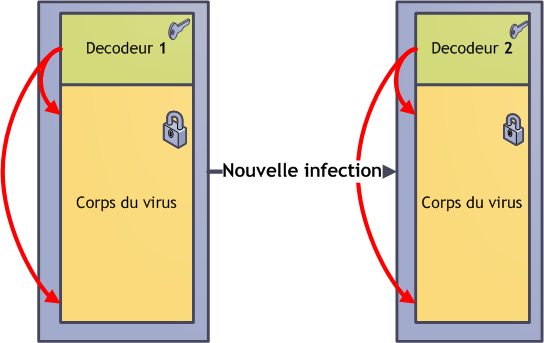
\includegraphics[scale=0.3]{olligo.png}
\center
\end{figure}
\end{column}
\end{columns}
\end{frame}

\begin{frame}{A votre avis}
\begin{itemize}
\item \huge{Quelles contremesures possibles ?}
\end{itemize}
\end{frame}


\begin{frame}{Le polymorphisme}
\begin{columns}[t]
\begin{column}{5cm}
\begin{exampleblock}{Le polymorphisme}
\begin{itemize}
\item Muter le code du décodeur à chaque génération
\item Code différent mais fonctionnement équivalent
\item Premier virus polymorphique: \texttt{1260} (1990)
\end{itemize}
\end{exampleblock}
\end{column}
\begin{column}{5cm}
\begin{figure}[!ht]
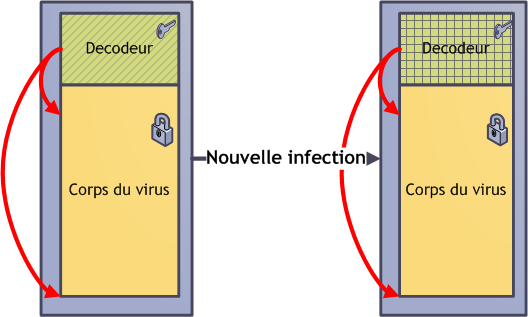
\includegraphics[scale=0.31]{poly.png}
\center
\end{figure}
\end{column}
\end{columns}
\end{frame}

\begin{frame}{Mutation de code}
Quelques mutations possibles:
\begin{itemize}
\item Insertion de code mort
\item Réorganisation (géographique) du code
\item Mutations syntaxiques (cf. TP)
\begin{itemize}
\item Utilisation de registres différents
\item Utilisation d'opcodes différents
\end{itemize}
\item Modification du CFG
\item ... et beaucoup d'autres
\end{itemize}
\begin{exampleblock}{}
\texttt{A Taxonomy of Obfuscating Transformations - C.Collberg}
\end{exampleblock}
\end{frame}


\begin{frame}[fragile]
\begin{exampleblock}{Un décrypteur de 1260}
\begin{lstlisting}[basicstyle=\tiny]
inc     si        ; optional, variable junk
mov     ax,0E9B   ; set key 1
clc               ; optional, variable junk
mov     di,012A   ; offset of Start
nop               ; optional, variable junk
mov     cx,0571   ; this many bytes - key 2
; Group 2  Decryption Instructions
Decrypt:
xor     [di],cx   ; decrypt first word with key 2
sub     bx,dx     ; optional, variable junk
xor     bx,cx     ; optional, variable junk
sub     bx,ax     ; optional, variable junk
sub     bx,cx     ; optional, variable junk
nop               ; non-optional junk
xor     dx,cx     ; optional, variable junk
xor     [di],ax   ; decrypt first word with key 1
; Group 3  Decryption Instructions
inc     di        ; next byte
nop               ; non-optional junk
clc               ; optional, variable junk
inc     ax        ; slide key 1
; loop
loop    Decrypt   ; until all bytes are decrypted  slide key 2
; random padding up to 39 bytes
Start:
;     Encrypted/decrypted virus body
\end{lstlisting} 
\end{exampleblock}
\end{frame}

\begin{frame}[fragile]{Démo}
\begin{alertblock}{Démonstration}
\begin{itemize}
\item Code source: 
 \begin{lstlisting}
	push 0xDEADBEEF
	push 0xDEADBABE
\end{lstlisting}
\item Mutation du code
\end{itemize}
\end{alertblock}
\end{frame}

\begin{frame}{A votre avis}
\begin{itemize}
\item \huge{Quelles contremesures possibles ?}
\end{itemize}
\end{frame}

\begin{frame}{Le metamorphisme}
\begin{columns}[t]
\begin{column}{5cm}
\begin{exampleblock}{Le metamorphisme}
\begin{itemize}
\item Plus de décodeur, trop "voyants"
\item Polymorphisme de tout le virus
\item Parfois metamorphisme de l'hôte
\item Premier virus métamorphique: \texttt{Regswap} (1998)
\end{itemize}
\end{exampleblock}
\end{column}
\begin{column}{5cm}
\begin{figure}[!ht]
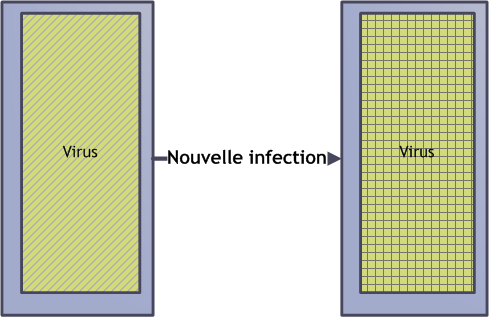
\includegraphics[scale=0.31]{meta.png}
\center
\end{figure}
\end{column}
\end{columns}
\end{frame}

\begin{frame}{Zmist}
Zmist par Zombie (2000)
\begin{itemize}
\item Virus métamorphique 
\begin{itemize}
\item mutations syntaxiques
\item modification du CFG
\end{itemize}
\item Intégration du virus dans l'hôte
\begin{itemize}
\item Désassemblage de l'hôte
\item Relocation
\item Intégration du virus par îlots
\end{itemize}
\item Recompilation du nouvel exécutable
\item Détecté à 99,1\% au bout de 7 ans
\end{itemize}
\end{frame}

\begin{frame}{A votre avis}
\begin{itemize}
\item \huge{Quelles contremesures possibles ?}
\end{itemize}
\end{frame}

\subsection{Détection}

\begin{frame}{Le problème de détection}
\begin{itemize}
\item Virus chiffrés simples ou oligomorphiques $\Rightarrow$ détection par signature sur le décodeur
\begin{itemize}
\item Au plus, $N$ signatures nécessaires
\end{itemize}
\item Technique \textit{X-Ray}
\begin{itemize}
\item Cryptanalyse automatisée pour les chiffrement les plus simples
\item Détection du \textbf{corps} du virus
\end{itemize}
\item Heuristique
\item Virus polymorphiques \textbf{simples} $\Rightarrow$ détection par signature\textbf{s}
\end{itemize}
\end{frame}


\begin{frame}{Le problème de détection (2)}
\begin{itemize}
\item Virus poly/métamorphiques complexes ?
\begin{itemize}
\item Une infinité de décodeurs peut être générée
\item On parle du \textbf{langage} du moteur de poly/métamorphisme
\item Symboles terminaux $\Leftrightarrow$ instructions machines
\end{itemize}
\item \textbf{Détection} du virus $\simeq$ \textbf{reconnaissance de ce langage}
\item Quelle complexité ?
\item Un peu de théorie ...
\end{itemize}
\end{frame}

\begin{frame}{Hiérarchie des langages formels}
\begin{figure}[!ht]
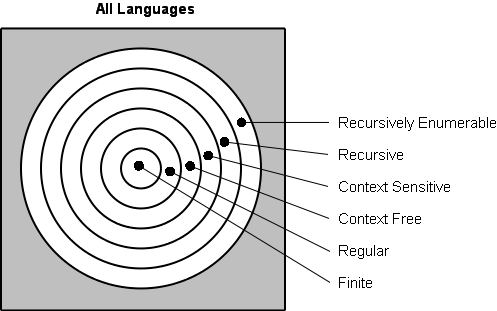
\includegraphics[scale=0.35]{chomsky.png}
\center
\caption{Langages formels}
\end{figure}
\end{frame}


\begin{frame}{Hierarchie des langages et complexité}
\begin{figure}[!ht]
\center
\tiny{
\begin{tabular}{|c|c|c|c|c|}
\hline
\textbf{Chomsky level} & \textbf{Grammaire} & \textbf{Langage} & \textbf{Autom. min.} & \textbf{Complexité}\\
\hline
Type 0 & Unrestricted & Recursively enumlerable & Turing machine\footnote{qui peut ne pas s'arrêter} & -\\
\hline
- & - & Recursive & Decider & ? \\
\hline
Type 1 & Contexte-sensitive & Contexte sensitive & Linear bounded TM & ?\\
\hline
- & Tree adjoining & Middly context-sensitive & Embedded pushdown & $P$\\
\hline
Type 2 & Context-free & Context-free & Nondet. pushdown & ?\\
\hline
- & $LL(k)$\footnote{et $LR(k)$ ...} & $LL(k)$ & Det. lookahead pushdown & ?\\
\hline
- & Det. context-free & Det. context-free & Det. pushdown & ?\\
\hline
Type 3 & Regular & Regular & DFA & ? \\
\hline
- & - & Star-free & Aperiodic finite & ?\\
\hline
\end{tabular}}
\end{figure}
\begin{itemize}
\item \texttt{mov reg,cst} $\Rightarrow$ \texttt{nop  ;  mov reg,cst} ?
\item \texttt{mov reg,cst} $\Rightarrow$ \texttt{push reg2 ; mov reg2,cst;  mov reg,reg2 ; pop reg2} ?
\end{itemize}
\end{frame}

\begin{frame}[fragile]{Le problème de détection (3)}
\begin{itemize}
\item Le problème de détection général est \textbf{indécidable}, que faire ?
\item Heuristique
\item Une détection exacte n'est pas obligatoire
\begin{itemize}
\item Détection de séquences d'instructions \textbf{suspectes} (signature)
\end{itemize}
\item Analyse statistique des instructions
\end{itemize}
\begin{exampleblock}{Scan antivir}
\tiny{
\begin{verbatim}
C:\taf\cours\09-10\lp\secu\cours\virus\demo1\testnotepad.exe
    [RESULTAT]  Contient le code suspect : GEN/Malware
    [REMARQUE]  Le résultat positif a été classé comme suspect.
\end{verbatim}}
\end{exampleblock}
\end{frame}

\begin{frame}{L'émulation}
\begin{itemize}
\item Pour les virus polymorphiques, le corps du virus \textbf{déchiffré} reste constant
\item Idée: \textbf{Emuler} le décodeur du virus 
\begin{itemize}
\item Interprétation du code machine instruction par instruction
\item Arrêt de l'émulateur à la fin du décodage
\end{itemize}
\item Le corps du virus apparaît en clair dans la VM de l'antivirus
\item $\Rightarrow$ signature sur le corps du virus
\end{itemize}
\end{frame}

\begin{frame}{L'émulation(2)}
\begin{figure}[!ht]
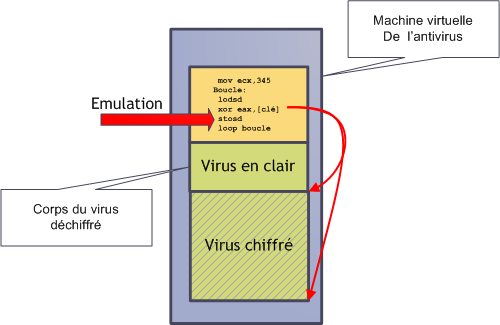
\includegraphics[scale=0.4]{emu.png}
\center
\caption{Emulation du décodeur du virus}
\end{figure}
\end{frame}


\begin{frame}{L'émulation: problèmes et solutions}
\begin{itemize}
\item Emuler du code est \textbf{lent} (et \textbf{non décidable})
\item Les virus tirent profit de cette lenteur:
\begin{itemize}
\item Insertion de code inutile long à émuler
\item Insertion d'instructions non supportées par l'émulateur
\end{itemize}
\item Contre-mesures:
\begin{itemize}
\item Suppression du code mort
\item Exécution des boucles \textbf{inoffensives} en \textbf{natif} (\textit{code normalization})
\end{itemize}
\end{itemize}
\end{frame}

\begin{frame}{La détection comportementale}
\begin{itemize}
\item Virus métamorphiques complexes: que faire ?
\item L'antivirus détourne les principaux appels systèmes
\item A l'\textbf{exécution} d'un programme, la séquence d'appels système est vérifiée
\begin{itemize}
\item Détection de sous-séquence d'appels systèmes suspects (\texttt{FindFirstFile(*.exe), WriteFile ...})
\item Détection de fréquences d'appels systèmes suspects
\end{itemize}
\item Avantage: très efficace contre les vers/trojans (API réseau)
\item Inconvénients:
\begin{itemize}
\item Ralentit le système de l'utilisateur
\item Détection parfois trop tardive
\end{itemize}
\end{itemize}
\begin{exampleblock}{Détection comportementale}
Malware behaviour analysis \textit{Wagener, G. and State, R. and Dulaunoy, A.} - 2008
\end{exampleblock}
\end{frame}


\begin{frame}{Etat de l'art}
Etat de l'art:
\begin{itemize}
\item Signature + heuristique + émulation
\item Heuristique au sein de l'émulateur
\begin{itemize}
\item Détection d'accès séquentiel au code du programme
\item Détection de routines virales classiques (scan *.exe, etc.)
\item Code auto-modifiant
\end{itemize}
\item Sandboxing (expérimental): émulation de l'os en entier
\item la majorité des virus sont détectés sans mise à jour de l'antivirus
\end{itemize}
\end{frame}

\section{Conclusion}

\subsection{Actuellement}
\begin{frame}{Actuellement}
\begin{itemize}
\item L'augmentation de la fréquence des CPU joue en faveur des antivirus
\begin{itemize}
\item Capacité d'émulation augmentée
\end{itemize}
\item L'augmentation de la taille des disques et du débit réseau joue en faveur des virus
\begin{itemize}
\item Plus complexes
\end{itemize}
\item Néanmoins:
\begin{itemize}
\item Les virus restent majoritairement détectés dès leur sortie
\item Très peu de virus innovants actuellement
\item Arrestations massives il y a 4-5 ans (29A)
\end{itemize}
\end{itemize}
\end{frame}


\subsection{Perspectives}
\begin{frame}{Changement sociologiques}
\begin{itemize}
\item Presque plus de vxers hobbyistes
\item La mode est au \textbf{profit}
\begin{itemize}
\item Equipe de plusieurs programmeurs
\item Réutilisation des techniques de virologie
\item Ajout de propagation via le réseau (mix virus/vers/botnets)
\end{itemize}
\item Une faille = un vers lancé sous deux semaines
\item Objectif: spam $\Rightarrow$ profit
\end{itemize}
\begin{exampleblock}{La rentabilité des botnets}
\textit{Spamalytics: An Empirical Analysis of Spam Marketing Conversion}\\ \url{http://www.icsi.berkeley.edu/pubs/networking/2008-ccs-spamalytics.pdf}
\end{exampleblock}
\end{frame}

\begin{frame}{Récapitulatif}
\begin{figure}[!ht]
\begin{tabular}{|c|c|}
\hline
\textbf{Attaque} & \textbf{Défense} \\
\hline
Virus boot & Signature \\
\hline
Infecteur de fichier & 	Signature, heuristique \\
\hline
Polymorphisme & Émulation+Signature, heuristique \\
\hline
Metamorphisme & Détection comportementale, heuristique \\
\hline
Vers, chevaux de troie & Détection comportementale, signature \\
\hline
\end{tabular}
\center
\end{figure}
\begin{itemize}
\item La \textbf{quasi totalité des techniques} des rootkits, vers, trojans et shellcodes \textbf{sont issues des virus}
\end{itemize}
\end{frame}

\end{document}